%%%%% Don't Make Changes Below Here %%%%%
\documentclass{article}\usepackage[utf8]{inputenc}\usepackage[margin=0.4cm,top=0.4cm,bottom=0.4cm]{geometry}\usepackage[usenames,dvipsnames,svgnames,table]{xcolor}\usepackage{bm}\usepackage{calligra}\usepackage{tikz, listings}\usepackage{hyperref}\usetikzlibrary{matrix,fit,chains,calc,scopes}\usepackage{tcolorbox}\tcbuselibrary{skins}\tcbset{Baystyle/.style={sharp corners,enhanced,boxrule=6pt,colframe=orange,height=\textheight,width=\textwidth,borderline={8pt}{-11pt}{},}}\usepackage{amsmath,amssymb,amsthm,tikz,tkz-graph,color,chngpage,soul,hyperref,csquotes,graphicx,floatrow}\newcommand*{\QEDB}{\hfill\ensuremath{\square}}\newtheorem*{prop}{Proposition}\renewcommand{\theenumi}{\alph{enumi}}\usepackage[shortlabels]{enumitem}\usetikzlibrary{matrix,calc}\MakeOuterQuote{"}\newtheorem{theorem}{Theorem} \usetikzlibrary{shapes} \usepackage{lipsum}\usepackage{tabularx,ragged2e,booktabs,caption}\tcbuselibrary{breakable}\newenvironment{yframed}{\begin{tcolorbox}[breakable,colback=gray!3,title after break={\textit{\color{red}Solution (cont.)}},colbacktitle=gray!3, coltitle=black,titlerule=-1pt] }{\end{tcolorbox}}\newtcolorbox{mybox}{colback=black!15!white, colframe=white,arc=12pt}\newtcolorbox{myboxot}{colback=green!15!white, colframe=white,arc=12pt,width=110pt, height=27pt}\newtcbox{\mylib}{enhanced,boxrule=0pt,top=0mm,bottom=0mm,right=0mm,left=4mm,arc=4pt,boxsep=9pt,before upper={\vphantom{dlg}},colframe=green!50!black,coltext=green!25!black,colback=green!10!white,overlay={\begin{tcbclipinterior}\fill[green!75!blue!50!white] (frame.south west)rectangle node[text=white,font=\sffamily\bfseries\tiny,rotate=90] {Problem} ([xshift=4mm]frame.north west);\end{tcbclipinterior}}}\newtcbox{\mylibot}{enhanced,boxrule=0pt,top=0mm,bottom=0mm,right=0mm,arc=4pt,boxsep=9pt,before upper={\vphantom{dlg}},colframe=green!50!black,coltext=green!25!black,colback=green!10!white,overlay={\begin{tcbclipinterior}\fill[red!75!blue!50!white] (frame.south west)rectangle node[text=white,font=\sffamily\bfseries\tiny,rotate=90] {Other} ([xshift=4mm]frame.north west);\end{tcbclipinterior}}}
\def\Title{\begin{tcolorbox}[Baystyle,]{\begin{center}\vspace*{0.14\textheight}
{\rule{\textwidth}{1.6pt}\vspace*{-\baselineskip}\vspace*{2pt}}
\rule{\textwidth}{0.4pt}\\[0.2\baselineskip]{\fontsize{45}{45}\scshape CS 189: Introduction to Machine Learning \\[0.2\baselineskip] \calligra Spring 2018 \\[0.2\baselineskip]}
{\rule{\textwidth}{0.4pt}\vspace*{-\baselineskip}\vspace{3.2pt}}
\rule{\textwidth}{1.6pt}\\[\baselineskip]\vspace{0.05\textheight}{{\fontsize{45}{45}\scshape$\bullet$\\ {Homework 5}\\\vspace*{0.01\textheight} }{{\fontsize{18}{18}\scshape{Due on Friday, February 23th, 2018 at 10pm\\}}}\fontsize{45}{45}\scshape$\bullet$  \\}\vspace*{0.1\textheight}{\fontsize{12}{12}\calligra Solutions by\\}{\fontsize{28}{28}\scshape \Name \\}\vspace*{0.01\textheight}{\fontsize{12}{12}\scshape \SID} \\\vspace*{0.05\textheight}{\fontsize{12}{12}\calligra In collaboration with\\}\vspace*{0.01\textheight}{\fontsize{12}{12}\scshape \Collabs} \\\vspace*{0.05\textheight}\end{center}}\end{tcolorbox}\newgeometry{margin=0.75in}}\def\BeginSolution{\begin{yframed}\textbf{\color{red}Solution }}\def\EndSolution{\end{yframed}}\usepackage{algorithm}\usepackage[noend]{algpseudocode}\makeatletter\def\BState{\State\hskip-\ALG@thistlm}\makeatother\def\star{\bigstar}\usetikzlibrary{arrows}\usepackage[mathscr]{euscript}\usepackage[T1]{fontenc}\DeclareSymbolFont{rsfs}{U}{rsfs}{m}{n}\DeclareSymbolFontAlphabet{\mathscrsfs}{rsfs}\newcommand\tab[1][1cm]{\hspace*{#1}}\hypersetup{colorlinks=true,urlcolor=blue}\newtheorem{lemma}[theorem]{Lemma}\newcommand{\norm}[1]{\left\lVert#1\right\rVert}\def\vec{\mathbf}\def\y{\mathbf{y}}\def\X{\mathbf{X}}\def\R{\mathbb{R}}\def\x{\mathbf{x}}\def\w{\mathbf{w}}\def\T{^\top}\def\r{\mathbf{r}}\def\mat{\mathbf}\def\I{\mathbf{I}}\def\A{\mathbf{A}}\newcommand{\num}{n}\newcommand{\dims}{d}\def\real{\mathbb{R}}
%%%%% Don't Make Changes Above Here %%%%%

%%%%% Template Begins Here %%%%%

\def\Name{Firstname Lastname}  % Your name
\def\SID{Student ID}  % Your student ID number
\def\Collabs{None} % Your collaborators here with a comma between each person's name. Write None if no collaborators. Don't leave blank.


\pagestyle{empty}
\begin{document}
\Title
\clearpage

%%%% Problem 1 Starts Here %%%%
\vspace{-2mm}\noindent\begin{mybox}{\begin{center}\textbf{\color{black}Problem 1: Getting Started}\end{center}}\end{mybox}\vspace{-2mm}
\vspace{10pt}
\noindent \textbf{Read through this page carefully.} You may typeset your homework in latex or submit neatly handwritten/scanned solutions. Please start each question on a new page. Deliverables:
\begin{enumerate}[1.]
\item Submit a PDF of your writeup, \textbf{with an appendix for your code}, to assignment on Gradescope, ``HW5 Write-Up''. If there are graphs, include those graphs in the correct sections. Do not simply reference your appendix.
\item If there is code, submit all code needed to reproduce your results, ``HW5 Code''.
\item If there is a test set, submit your test set evaluation results, ``HW5 Test Set''.
\end{enumerate}
After you've submitted your homework, watch out for the self-grade form.
\begin{enumerate}
\item Who else did you you work with on this homework? In case of course events, just describe the group. How did you work on this homework? Any comments about the homework?
\BeginSolution
%1a

\EndSolution
\item Please copy the following statement and sign next to it. We just want to make it \textit{extra} clear so that no one inadvertently cheats.

\textit{I certify that all solutions are entirely in my words and that I have not looked at another student's solutions. I have credited all external sources in this write up.}
\BeginSolution
%1b

\EndSolution
\end{enumerate}
%%%% Problem 1 Ends Here %%%%
\clearpage

%%%% Problem 2 Starts Here %%%%
\vspace{-2mm}\noindent\begin{mybox}{\begin{center}\textbf{\color{black}Problem 2: Total Least Squares}\end{center}}\end{mybox}\vspace{-2mm}
\vspace{10pt}
\noindent In most of the models we have looked at so far, we've accounted for noise in the observed y measurement and adjusted accordingly. However, in the real world it could easily be that our feature matrix X of data is also corrupted or noisy. Total least squares is a way to account for this. Whereas previously we were minimizing the y distance from the data point to our predicted line because we had assumed the features were definitively accurate, now we are minimizing the entire distance from the data point to our predicted line. In this problem we will explore the mathematical intuition for the TLS formula. We will then apply the formula to adjusting the lighting of an image which contains noise in its feature matrix due to inaccurate assumptions we make about the image, such as the image being a perfect sphere.
\vspace{4pt}

\noindent Let $\mat{X}$ and $\vec{y}$ be the true measurements. Recall that in the least squares problem, we want to solve for $\vec{w}$ in $\min_{\vec{w}}{||\mat{X}\vec{w}-\vec{y}||}$. We measure the error as the difference between $\mat{X}\vec{w}$ and $\vec{y}$, which can be viewed as adding an error term $\vec{\epsilon_y}$ such that the equation $\mat{X}\vec{w}=\vec{y}+\vec{\epsilon_y}$ has a solution \begin{align}\min_{\vec{\epsilon_y}, \vec{w}} \lvert\lvert\vec{\epsilon_y}\rvert\rvert_2,\text{ subject to }\mat{X}\vec{w}=\vec{y}+\vec{\epsilon_y} \label{eq:ls_min} \end{align}Although this optimization formulation allows for errors in the measurements of $\vec{y}$, it does not allow for errors in the feature matrix $\mat{X}$ that is measured from the data.  In this problem, we will explore a method called \emph{total least squares} that allows for both error in the matrix $\mat{X}$ and the vector $\vec{y}$, represented by $\mat{\epsilon_X}$ and $\vec{\epsilon_y}$, respectively. For convenience, we absorb the negative sign into $\vec{\epsilon_y}$ and $\vec{\epsilon_X}$ and define true measurements $\vec{y}$ and $\vec{X}$ like so:\begin{align}\vec{y}^{true} = \vec{y} + \vec{\epsilon_y} \\\mat{X}^{true} = \mat{X} + \mat{\epsilon_X} \end{align} Specifically, the total least squares problem is to find the solution for $\vec{w}$ in the following minimization problem:\begin{align}\min_{\vec{\epsilon_y}, \vec{\epsilon_X}, \vec{w}} \lvert\lvert[\mat{\epsilon_X},\vec{\epsilon_y}]\rvert\rvert^2_F,\text{ subject to }(\mat{X}+\mat{\epsilon_X})\vec{w}=\vec{y}+\vec{\epsilon_y}\label{eq:tls_min}\end{align}where the matrix $[\mat{\epsilon_X},\vec{\epsilon_y}]$ is the concatenation of the columns of $\mat{\epsilon_X}$ with the column vector $\vec{y}$. Notice that the minimization is over $\vec{w}$ because it's a free parameter, and it does not necessarily have to be in the objective function. Intuitively, this equation is finding the smallest perturbation to the matrix of data points $\mat{X}$ and the outputs $\vec{y}$ such that the linear model can be solved exactly. The constraint in the minimization problem can be rewritten as \begin{align}[\mat{X}+\mat{\epsilon_X},\vec{y}+\vec{\epsilon_y}]\begin{bmatrix}\vec{w}\\-1\end{bmatrix}=\vec{0}	\label{eq:tls}\end{align}
\begin{enumerate}
\item Let the matrix $\mat{X}\in\mathbb{R}^{n\times d}$ and $\vec{y}\in\mathbb{R}^n$ and note that $\epsilon_{X}\in\mathbb{R}^{n\times d}$ and $\vec{\epsilon_y}\in\mathbb{R}^n$.  Assuming that $n>d$ and $\text{rank}(\mat{X}+\mat{\epsilon_X})=d$, \textbf{explain why  $\text{rank}([\mat{X}+\mat{\epsilon_X},\vec{y}+\vec{\epsilon_y}])=d$.}
\BeginSolution
%2a

\EndSolution
\item For the solution $\vec{w}$ to be unique, the matrix $[\mat{X}+\mat{\epsilon_X},\vec{y}+\vec{\epsilon_y}]$ must have exactly d linearly independent columns. Since this matrix has d+1 columns in total, it must be rank-deficient by 1. Recall that the Eckart-Young-Mirsky Theorem tells us that the closest lower-rank matrix in the Frobenius norm is obtained by discarding the smallest singular values. Therefore, the matrix $[\mat{X}+\mat{\epsilon_X},\vec{y}+\vec{\epsilon_y}]$ that minimizes $$\lvert\lvert[\mat{\epsilon_X},\vec{\epsilon_y}]\rvert\rvert^2_F = \lvert\lvert[\mat{X}^{true},\vec{y}^{true}] - [\mat{X},\vec{y}] \rvert\rvert^2_F$$ is given by\begin{align*}[\mat{X}+\mat{\epsilon_X},\vec{y}+\vec{\epsilon_y}]&=U\begin{bmatrix}\Sigma_{d}&\\&0\end{bmatrix}V^\top\end{align*}where $ [\mat{X},\vec{y}]=U\Sigma V^\top$ and $\Sigma_{d}$ is the diagonal matrix of the $d$ largest singular values of $[\mat{X},\vec{y}]$.  
\vspace{4pt}

\noindent Suppose we express the SVD of $[\mat{X},\vec{y}]$ in terms of submatrices and vectors:\begin{align*}[\mat{X},\vec{y}] = \begin{bmatrix}\mat{U}_{xx}&\vec{u}_{xy}\\\vec{u}_{xy}^\top&u_{yy}\end{bmatrix}\begin{bmatrix}\Sigma_{d}&\\&\sigma_{d+1}\end{bmatrix}\begin{bmatrix}\mat{V}_{xx}&\vec{v}_{xy}\\\vec{v}_{xy}^\top&v_{yy}\end{bmatrix}^\top\end{align*}where the vectors $\vec{u}_{xy} \in\mathbb{R}^{d}$ and $\vec{v}_{xy} \in\mathbb{R}^{d}$ are the first d elements of the (d+1)-th column of $\mat{U}$ and $\mat{V}$ respectively, $u_{yy}$ and $v_{yy}$ are the (d+1)-th element of the d+1 column of $\mat{U}$ and $\mat{V}$ respectively, $\mat{U}_{xx} \in\mathbb{R}^{d\times d}$ and $\mat{V}_{xx} \in\mathbb{R}^{d\times d}$ are the $d \times d$ top left submatrices of $\mat{U}$ and $\mat{V}$ respectively, and  $\sigma_{d+1}$ is the (d+1)-th eigenvalue of $[\mat{X},\vec{y}]$.
\vspace{4pt}

\noindent \textbf{Using this information show that}\begin{align*}[\mat{\epsilon_X},\vec{\epsilon_y}]&=- \begin{bmatrix}\vec{u}_{xy}\\u_{yy}\end{bmatrix}\sigma_{d+1}\begin{bmatrix}\vec{v}_{xy}\\v_{yy}\end{bmatrix}^\top\end{align*}
\BeginSolution
%2b

\EndSolution
\item \textbf{Using the result from the previous part and that fact that $v_{yy}$ is not 0 (see notes on Total Least Squares), find a nonzero solution to $[\mat{X}+\mat{\epsilon_X},\vec{y}+\vec{\epsilon_y}]\begin{bmatrix}\vec{w}\\-1\end{bmatrix}=\vec{0}$ and thus solve for $\vec{w}$ in Equation~\eqref{eq:tls}.}
\vspace{4pt}

\noindent \emph{HINT: Looking at the last column of the product $[\mat{X},\vec{y}]\mat{V}$ may or may not be useful for this problem, depending on how you solve it.}
\BeginSolution
%2c

\EndSolution
\item From the previous part, you can see that $\begin{bmatrix}\vec{w}\\-1\end{bmatrix}$ is a right-singular vector of $[\mat{X},\vec{y}]$. \textbf{Show that $$(\X^\top \X - \sigma_{d+1}^2 I)\vec{w} = \X^\top\y \eqno(14)$$}
\BeginSolution
%2d

\EndSolution
\item In this problem, we will use total least squares to approximately learn the lighting in a photograph, which we can then use to paste new objects into the image while still maintaining the realism of the image.  You will be estimating the lighting coefficients for the interior of St.~Peter's Basillica, and you will then use these coefficients to change the lighting of an image of a tennis ball so that it can be pasted into the image.  In Figure~\ref{fig:noshade}, we show the result of pasting the tennis ball in the image without adjusting the lighting on the ball.  The ball looks too bright for the scene and does not look like it would fit in with other objects in the image. \begin{figure}[h]\centering\begin{minipage}[b]{0.4\textwidth}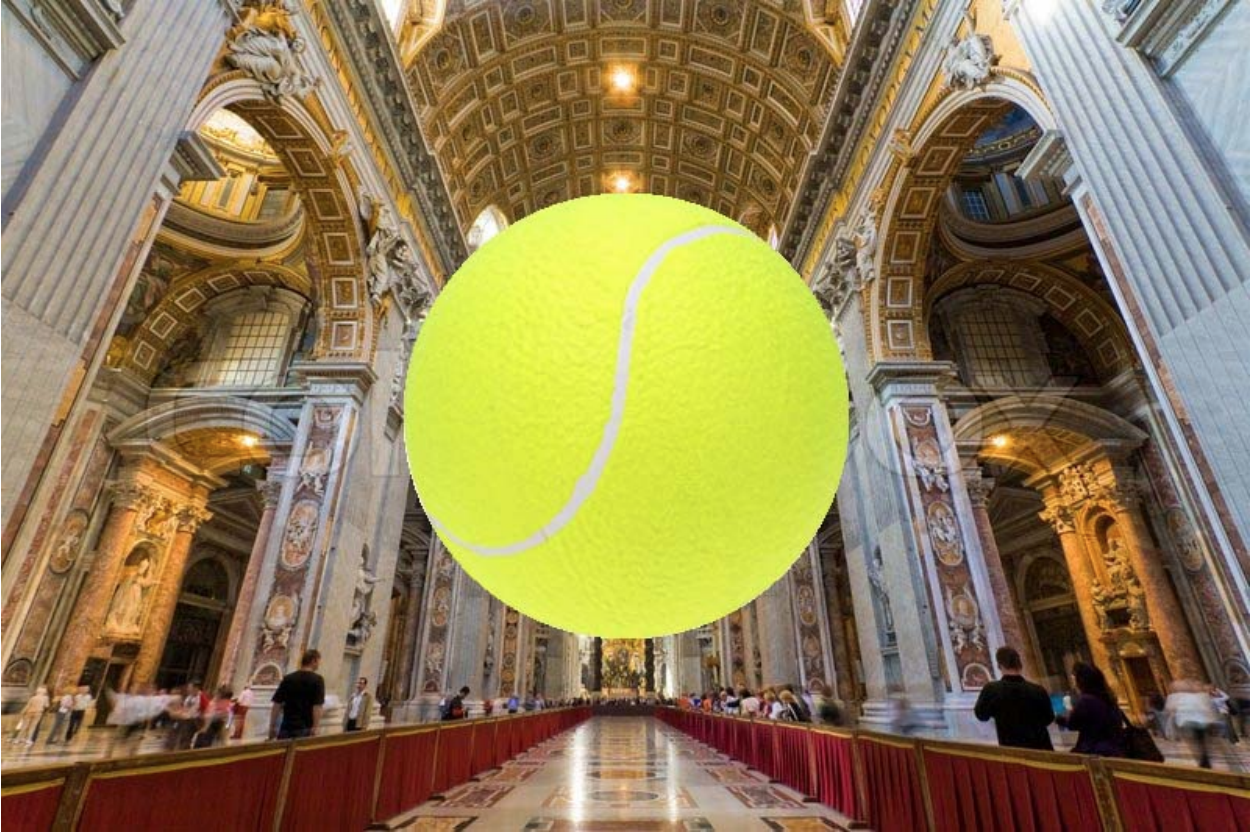
\includegraphics[width=\textwidth]{tennis_no_shade}\end{minipage}\begin{minipage}[b]{0.4\textwidth}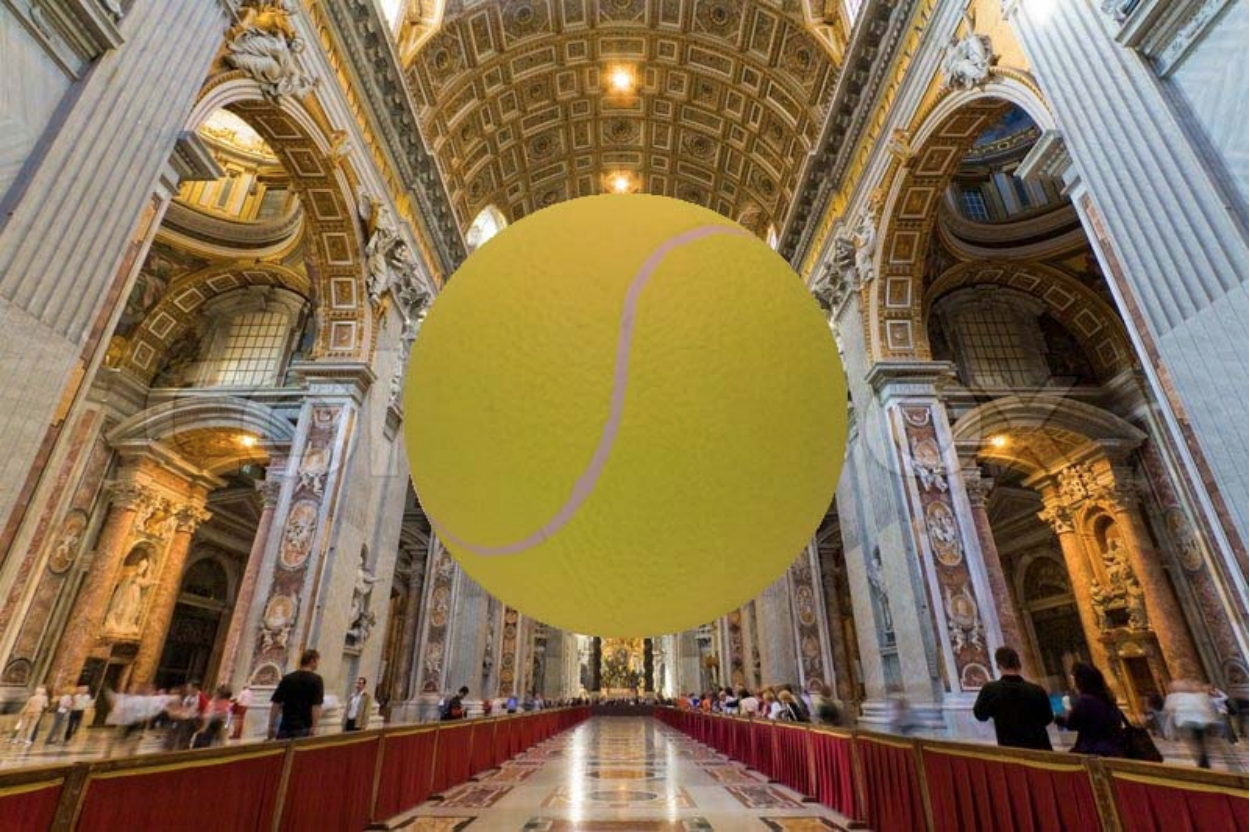
\includegraphics[width=\textwidth]{tennis_lsq}\end{minipage}\caption{Tennis ball pasted on top of image of St.~Peter's Basillica without lighting adjustment (left) and with lighting adjustment (right)}\label{fig:noshade}\end{figure} To convincingly add a tennis ball to an image, we need to need to apply the appropriate lighting from the environment onto the added ball.  To start, we will represent environment lighting as a spherical function $\vec{f}(\vec{n})$ where $\vec{n}$ is a 3 dimensional unit vector ($\lvert\lvert\vec{n}\rvert\rvert_2=1$), and $\vec{f}$ outputs a 3 dimensional color vector, one component for red, green, and blue light intensities. Because $\vec{f}(\vec{n})$ is a spherical function, the input $\vec{n}$ must correspond to a point on a sphere. The function $\vec{f}(\vec{n})$ represents the total incoming light from the direction $\vec{n}$ in the scene.  The lighting function of a spherical object $\vec{f}(\vec{n})$ can be approximated by the first 9 spherical harmonic basis functions. 
\vspace{4pt}

\noindent The first 9 unnormalized sperical harmonic basis functions are given by: \begin{align*}L_{1}&=1\\L_{2}&=y\\L_{3}&=x\\L_{4}&=z\\L_{5}&=xy\\L_{6}&=yz\\L_{7}&=3z^2-1\\L_{8}&=xz\\L_{9}&=x^2-y^2\end{align*}where $\vec{n}=[x,y,z]^\top$.  The lighting function can then be approximated as\begin{align*}\vec{f}(\vec{n}) \approx\sum_{i=1}^9 \vec{\gamma}_i L_i(\vec{n})\end{align*} \[\begin{bmatrix}\text{ ---} & \vec{f}(\vec{n_1}) & \text{--- } \\\text{ ---} & \vec{f}(\vec{n_2}) & \text{--- } \\& \vdots & \\\text{ ---} & \vec{f}(\vec{n_n}) & \text{--- }\end{bmatrix}_{n \times 3}=\begin{bmatrix}L_1(\vec{n_1}) &L_2(\vec{n_1}) & ... & L_9(\vec{n_1}) \\L_1(\vec{n_2}) & L_2(\vec{n_2}) & ... & L_9(\vec{n_2}) \\& \vdots & \\L_1(\vec{n_n}) & L_2(\vec{n_n}) & ... & L_9(\vec{n_n}) \\\end{bmatrix}_{n \times 9}\begin{bmatrix}\text{ ---} & \vec{\gamma}_1 & \text{--- } \\\text{ ---} & \vec{\gamma}_2 & \text{--- } \\& \vdots & \\\text{ ---} & \vec{\gamma}_9 & \text{--- }\end{bmatrix}_{9 \times 3}\] where $L_i(\vec{n})$ is the $i$th basis function from the list above.
\vspace{4pt}

\noindent The function of incoming light $\vec{f}(\vec{n})$ can be measured by photographing a spherical mirror placed in the scene of interest.  In this case, we provide you with an image of the sphere as seen in Figure~\ref{fig:probe}. \begin{figure}[h]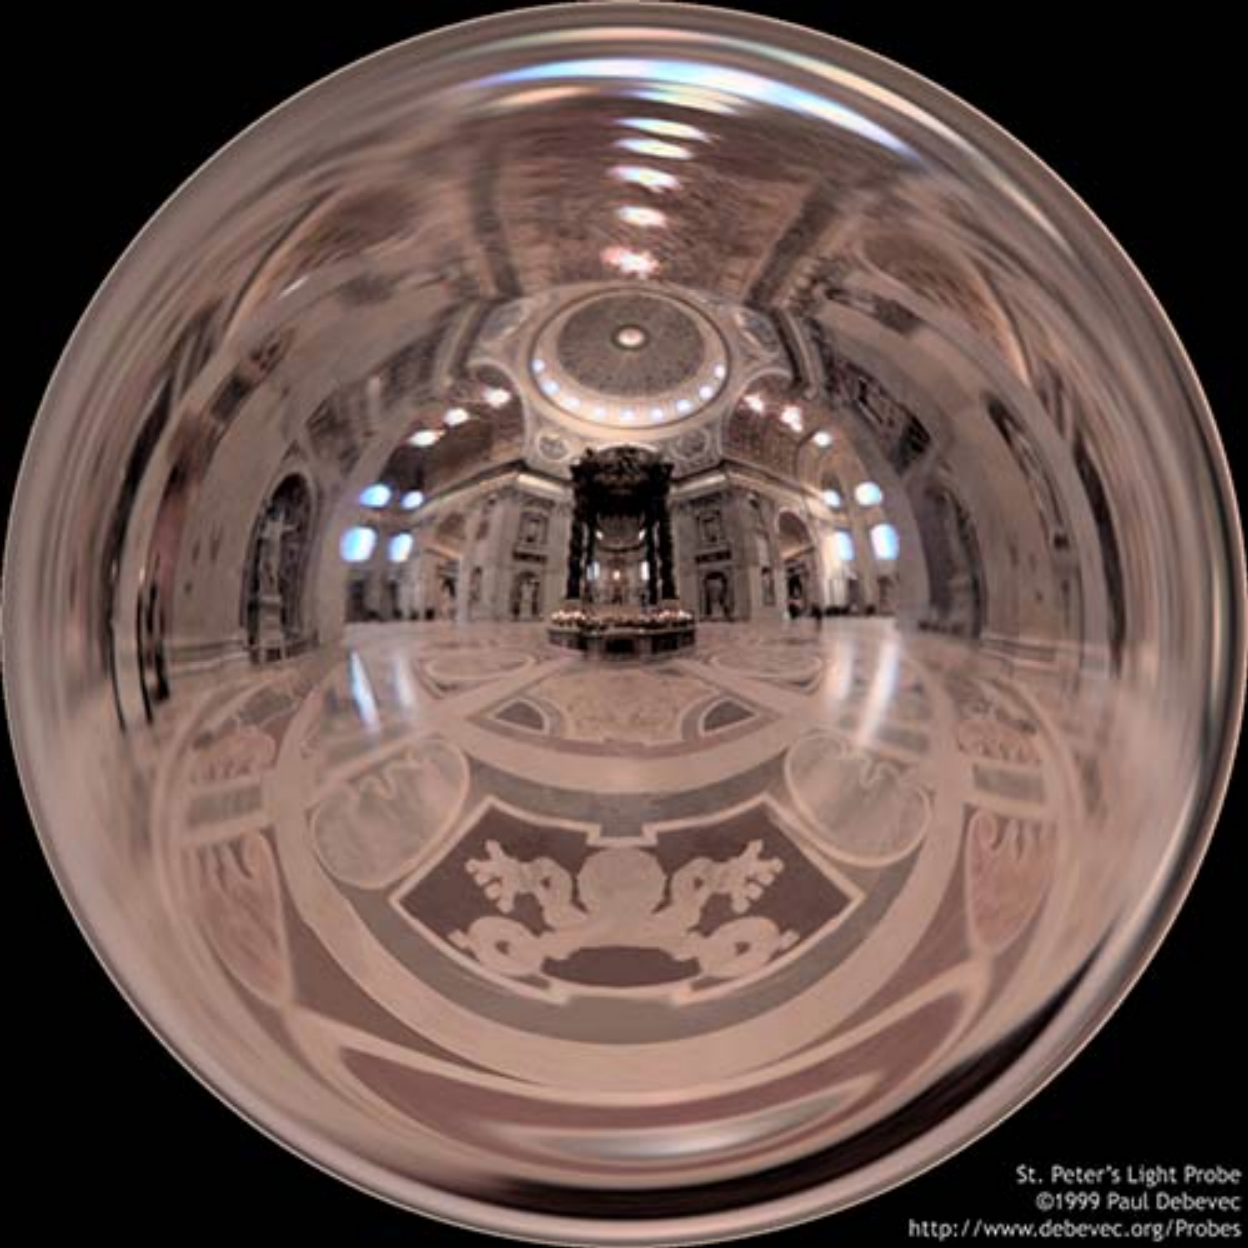
\includegraphics[width=0.4\textwidth]{stpeters_probe_small}\caption{Image of a spherical mirror inside of St. Peter's Basillica}\label{fig:probe}\end{figure} In the code provided, there is a function extractNormals(img) that will extract the training pairs $(\vec{n}_i,\vec{f}(\vec{n}_i))$ from the image.  An example using this function is in the code.
\vspace{4pt}

\noindent \textbf{Use the spherical harmonic basis functions to create a $9$ dimensional feature vector for each sample.  Use this to formulate an ordinary least squares problem and solve for the unknown coefficients $\vec{\gamma}_i$.  Report the estimated values for $\vec{\gamma}_i$ and include a visualization of the approximation using the provided code.} The code provided will load the images, extracts the training data, relights the tennis ball with incorrect coefficients, and saves the results.  Your task is to compute the basis functions and solve the least squares problems to provide the code with the correct coefficients.  To run the starter code, you will need to use Python with \texttt{numpy} and \texttt{scipy}.  Because the resulting data set is large, we reduce it in the code by taking every $50^\text{th}$ entry in the data.  This is done for you in the starter code, but you can try using the entire data set or reduce it by a different amount.
\BeginSolution
%2e

\EndSolution
\item When we extract from the data the direction $\vec{n}$ to compute  $(\vec{n}_i,\vec{f}(\vec{n}_i))$, we make some approximations about how the light is captured on the image.  We also assume that the spherical mirror is a perfect sphere, but in reality, there will always be small imperfections.  Thus, our measurement for $\vec{n}$ contains some error, which makes this an ideal problem to apply total least squares.  \textbf{Solve this problem with total least squares by allowing perturbations in the matrix of basis functions.  Report the estimated values for $\vec{\gamma}_i$ and include a visualization of the approximation.}  The output image will be visibly wrong, and we'll explore how to fix this problem in the next part.  Your implementation may only use the SVD and the matrix inverse functions from the linear algebra library in \texttt{numpy}.
\BeginSolution
%2f

\EndSolution
\item In the previous part, you should have noticed that the visualization is drastically different than the one generated using least squares. Recall that in total least squares we are minimizing  $\lvert\lvert[\mat{\epsilon_X},\vec{\epsilon_y}]\rvert\rvert^2_F$. Intuitively, to minimize the Frobenius norm of components of both the inputs and outputs, the inputs and outputs should be on the same scale. However, this is not the case here. Color values in an image will typically be in $[0,255]$, but the original image had a much larger range.  We compressed the range to a smaller scale using tone mapping, but the effect of the compression is that relatively bright areas of the image become less bright.  As a compromise, we scaled the image colors down to a maximum color value of $384$ instead of $255$. Thus, the inputs here are all unit vectors, and the outputs are 3 dimensional vectors where each value is in $[0,384]$.  \textbf{Propose a value by which to scale the outputs $\vec{f}(\vec{n}_i)$ such that the values of the inputs and outputs are roughly on the same scale. Solve this scaled total least squares problem, report the computed spherical harmonic coefficients and provide a rendering of the relit sphere.}
\BeginSolution
%2g

\EndSolution
\end{enumerate}
%%%% Problem 2 Ends Here %%%%
\clearpage

%%%% Problem 3 Starts Here %%%%
\vspace{-2mm}\noindent\begin{mybox}{\begin{center}\textbf{\color{black}Problem 3: PCA and Random Projections}\end{center}}\end{mybox}\vspace{-2mm}
\vspace{10pt}
\noindent In this question, we revisit the task of dimensionality reduction. Dimensionality reduction is useful for several purposes, including but not restricted to, visualization, storage, faster computation etc. While reducing dimension is useful, it is not undesirable to demand that such reductions preserve some properties of the original data. Often, certain geometric properties like distance and inner products are important to perform certain machine learning tasks. And as a result, we may want to perform dimensionality reduction but ensuring that we approximately maintain the pairwise distances and inner products.
\vspace{4pt}

\noindent While you have already seen many properties of PCA so far, in this question we investigate if random projections work are a good idea for dimensionality reduction. A few advantages of random projections over PCA can be listed as: \begin{enumerate}[1.]\item PCA is expensive when the underlying dimension is high and the number of principal components is also large (however note that there are several very fast algorithms dedicated to doing PCA), \item PCA requires you to have access to the feature matrix for performing computations. The second requirement of PCA is a bottle neck when you want to take only a low dimensional measurement of a very high dimensional data, e.g., in FMRI and in compressed sensing. In such cases, one needs to design a projection scheme before seeing the data. We now turn to a concrete setting study a few properties of PCA and random projections.\end{enumerate}
\vspace{4pt}

\noindent Suppose you are given $\num$ points $\vec x_1, \ldots, \vec x_\num$ in $\real^\dims$. Define the $\num \times \dims$ matrix $\mat X = \begin{bmatrix}\vec x_1^\top \\ \vdots \\ \vec x_\num^\top \end{bmatrix}$ where each row of the matrix represents one of the given points. In this problem, we will consider a few low-dimensional embedding $\psi: \real^\dims \mapsto \real^k$ that maps vectors from $\real^\dims$ to $\real^k$.
\vspace{4pt}

\noindent Let $\mat X = \mat U {\bm{\Sigma}} \mat V^\top$ denote the singular value decomposition of the matrix $\mat X$. Assume that $N \geq d$ and let $\sigma_1 \geq \sigma_2 \geq \ldots \geq \sigma_d$ denote the singular values of $\mat X$.
\vspace{4pt}

\noindent Let $\vec v_1, \vec v_2, \ldots, \vec v_d$ denote the columns of the matrix $\mat V$. We now consider the following $k$-dimensional PCA embedding:  $\psi_{\text{PCA}}(\vec x) = (\vec v_1^\top \vec x, \ldots, \vec v_k^\top \vec x)^\top$. Note that this embedding projects a $\dims$-dimensional vector on the linear span of the set $\{\vec v_1, \ldots, \vec v_k \}$ and that $\vec v_i^\top \vec x$ denotes the $i$-th coordinate of the projected vector in the new space.
\vspace{4pt}

\noindent We begin with a few matrix algebra relationships, and use it to investigate certain mathematical properties of PCA and random projections in the first few parts, and then see them in action on a synthetic dataset in the later parts.
\vspace{4pt}

\noindent {\bf Notation}: The symbol $[\num]$ stands for the set $\{1, \ldots, \num\}$.
\begin{enumerate}
\item {\bf What is the $ij$-th entry of the matrices $\mat X \mat X^\top$ and $\mat X^\top \mat X$? Express the matrix $\mat X \mat X^\top$ in terms of $\mat U$ and ${\bm \Sigma}$, and, express the matrix $\mat X^\top \mat X$  in terms of ${\bm \Sigma}$ and $\mat V$.}
\BeginSolution
%3a

\EndSolution
\item {\bf Show that }\begin{align*}\psi_{\text{PCA}}(\vec x_i)^\top\psi_\text{PCA}(\vec x_j) =  \vec x_i^\top\mat V_k\mat V_k^\top\vec x_j\quad\text{where}\quad\mat V_k = \begin{bmatrix}\vec v_1 & \vec v_2 & \ldots & \vec v_k\end{bmatrix}.\end{align*} Also {\bf show that $\mat V_k \mat V_k^\top = \mat V \mat I^k \mat V^\top$}, where the matrix $\mat I^k$ denotes a $\dims \times \dims$ diagonal matrix with first $k$ diagonal entries as $1$ and all other entries as zero.
\BeginSolution
%3b

\EndSolution
\item Suppose that we know the first $k$ singular values are the dominant singular values. In particular, we are given that\begin{align*}\frac{\sum_{i=1}^k \sigma_j^2}{\sum_{i=1}^d \sigma_i^2} \geq 1-\epsilon,\end{align*}for some $\epsilon \in (0, 1)$. Then {\bf show that the PCA projection to the first $k$-right singular vectorspreserves the \emph{inner products} on average:}\begin{align}\label{eq:pca_iprod}\frac{1}{\sum_{i=1}^\num\sum_{j=1}^\num(\vec x_i^\top\vec x_j)^2}\sum_{i=1}^\num \sum_{j=1}^\num \vert (\vec x_i^\top \vec x_j) - (\psi_{\text{PCA}}(\vec x_i)^\top \psi_{\text{PCA}}(\vec x_j)) \vert^2 \leq\epsilon.\end{align}Thus, we find that if there are dominant singular values, PCA projection can preserve the inner products on average. 
\vspace{4pt}

\noindent Hint: Using previous two parts and the definition of Frobenius norm might be useful.
\BeginSolution
%3c

\EndSolution
\item Now consider a different embedding $\psi:\real^\dims \mapsto \real^k$ which preserves all pairwise distances and norms up-to a multiplicative factor, that is, \begin{align}(1-\epsilon) \Vert \vec x_i \Vert^2 &\leq \Vert \psi(\vec x_i) \Vert^2 \leq (1+\epsilon) \Vert \vec x_i \Vert^2 \quad &\text{ for all } i \in [\num], \quad\text{and} \label{eq:norm}\\	(1-\epsilon) \Vert\vec x_i - \vec x_j \Vert^2 &\leq  \Vert \psi(\vec x_i) - \psi(\vec x_j) \Vert^2 	\leq (1+\epsilon) \Vert\vec x_i - \vec x_j \Vert^2 \quad &\text{ for all } i, j \in [\num], \quad \quad \label{eq:dist} \end{align} where $0<\epsilon \ll 1$ is a small scalar. Further assume that $\norm{\vec{x}_i} \leq 1$ for all $i \in [\num]$. {\bf Show that the embedding $\psi$ satisfying equations~\eqref{eq:dist} and \eqref{eq:norm} preserves \emph{each pairwise inner product}:}\begin{align}\label{eq:psi_iprod}\vert \psi(\vec x_i)^\top\psi(\vec x_j) - (\vec x_i^\top \vec x_j) \vert  \leq C\epsilon, \quad \text{ for all } i, j \in [\num],\end{align} {\bf for some constant $C$}. Thus, we find that if an embedding  approximately preserves distances and norms upto a small multiplicative factor, and the points have bounded norms, then inner products are also approximately preserved upto an additive factor.
\vspace{4pt}

\noindent Hint: You may use the Cauchy-Schwarz inequality.
\BeginSolution
%3d

\EndSolution
\item Now we consider the \emph{random projection} using a Gaussian matrix as introduced in the section. In next few parts, we work towards proving that if the dimension of projection is moderately big, then with high probability, the random projection preserves norms and pairwise distances approximately as described in equations~\eqref{eq:dist} and \eqref{eq:norm}.
\vspace{4pt}

\noindent Consider the random matrix $ \mat J \in \real^{k \times d}$ with each of its entry being i.i.d. $\mathcal{N}(0, 1)$ and consider the map $\psi_{\mat J}: \real^\dims \mapsto \real^k$ such that $\psi_{\mat J}(\vec{x})= \frac{1}{\sqrt{k}}\mat J \vec x$. {\bf Show that for any \emph{fixed non-zero vector $\vec u$}, the random variable $\displaystyle\frac{\Vert \psi_{\mat J}(\vec u)\Vert^2}{\Vert \vec u\Vert^2}$ can be written as \begin{align*}\frac{1}{k}\sum_{i=1}^k Z_i^2 \end{align*} where $Z_i$'s are i.i.d. $\mathcal{N}(0, 1)$ random variables.}
\BeginSolution
%3e

\EndSolution
\item For i.i.d. $Z_i \sim \mathcal{N}(0, 1)$, we have the following probability bound\begin{align*}\mathbb{P}\left[ \left\vert\frac{1}{k}\sum_{i=1}^k Z_i^2\right\vert \notin (1-t, 1+t) \right] \leq 2e^{-kt^2/8}, \quad \text{ for all } t \in (0, 1).\end{align*} Note that this bound suggests that $\sum_{i=1}^k Z_i^2 \approx \sum_{i=1}E[Z_i^2] = k$ with high probability. In other words, sum of square of Gaussian random variables concentrates around its mean with high probability. Using this bound and the previous part, now {\bf show that if $k \geq \frac{16}{\epsilon^2} \log\left(\frac{N}{\delta}\right)$, then }\begin{align*}\mathbb{P}\left[ \text{ for all } i, j \in [\num], i\neq j, \frac{\norm{\psi_{\mat J}(\vec x_i) - \psi_{\mat J}(\vec x_j)}^2}{\norm{\vec x_i - \vec x_j}^2} \in (1-\epsilon, 1+\epsilon) \right]\geq 1-\delta.\end{align*} That is show that for $k$ large enough, with high probability the random projection $\psi_{\mat J}$ approximately preserves the pairwise distances. Using this result, we can conclude that random projection serves as a good tool for dimensionality reduction if we project to enough number of dimensions. This result is popularly known as the \emph{Johnson-Lindenstrauss Lemma}.
\vspace{4pt}

\noindent Hint 1: The following (powerful technique cum) bound might be useful: For a set of events ${A_{ij}}$, we have \begin{align*}\mathbb{P}\left[ \cap_{i, j} A_{ij} \right]= 1- \mathbb{P}\left[ (\cap_{i, j} A_{ij})^c\right] = 1 - \mathbb{P}\left[ \cup_{i, j} A_{ij}^c\right] \geq 1 - \sum_{ij} \mathbb{P}\left[ A_{ij}^c\right].\end{align*}You may define the event $A_{ij} = \left\{\displaystyle\frac{\norm{\psi_{\mat J}(\vec x_i) - \psi_{\mat J}(\vec x_j)}^2}{\norm{\vec x_i - \vec x_j}^2} \in (1-\epsilon, 1+\epsilon) \right\}$ and use the union bound above.
\BeginSolution
%3f

\EndSolution
\item Suppose there are two clusters of points $S_1 = \{\vec u_1, \ldots, \vec u_n \}$ and $S_2 = \{\vec v_1, \ldots, \vec v_m \}$ which are far apart, i.e., we have \begin{align*}d^2(S_1, S_2) = \min_{u \in S_1, v \in S_2} \norm{u-v}^2 \geq \gamma.\end{align*}Then using the previous part, {\bf show that the random projection $\psi_{\mat J}$ also approximately maintains the distance between the two clusters if $k$ is large enough, that is, with high probability} \begin{align*}d^2(\psi_{\mat J}(S_1), \psi_{\mat J}(S_2)) = \min_{u \in S_1, v \in S_2}\norm{\psi_{\mat J}(\vec u) - \psi_{\mat J}(\vec v)}^2 \geq (1-\epsilon)\gamma \quad \text{if } k \geq \frac{C}{\epsilon^2} \log(m+n)\end{align*}for some constant $C$. Note that such a property can help in several machine learning tasks. For example, if the clusters of features for different labels were far in the original dimension, then this problem shows that even after randomly projecting the clusters they will remain far enough and a machine learning model may perform well even with the projected data. We now turn to visualizing some of these conclusions on a synthetic dataset.
\BeginSolution
%3g

\EndSolution
\item In the next few parts, we visualize the effect of PCA projections and random projections on a classification task. You are given 3 datasets in the data folder and a starter code.
\vspace{4pt}

\noindent Use the starter code to load the three datasets one by one. Note that there are two unique values in $\vec y$. {\bf Visualize the features of $\mat X$ these datasets using (1) Top-2 PCA components, and (2) 2-dimensional random projections. Use the code to project the features to $2$ dimensions and then scatter plot the $2$ features with a different color for each class.}Note that you will obtain $2$ plots for each dataset (total 6 plots for this part). {\bf Do you observe a difference in PCA vs random projections? Do you see a trend in the three datasets?}
\BeginSolution
%3h

\EndSolution
\item For each dataset, we will now fit a linear model on different projections of features to perform classification. The code for fitting a linear model with projected features and predicting a label for a given feature, is given to you. Use these functions and write a code that does prediction in the following way: (1) Use top $k$-PCA features to obtain one set of results, and (2) Use $k$-dimensional random projection to obtain the second set of results (take average accuracy over $10$ random projections for smooth curves). Use the projection functions given in the starter code to select these features. You should vary $k$ from $1$ to $d$ where $d$ is the dimension of each feature $\vec x_i$. {\bf Plot the accuracy for PCA and Random projection as a function of $k$. Comment on the observations on these accuracies as a function of $k$ and across different datasets.}
\BeginSolution
%3i

\EndSolution
\item ow plot the singular values for the feature matrices of the three datasets. {\bf Do you observe a pattern across the three datasets? Does it help to explain the performance of PCA observed in the previous parts?} 
\BeginSolution
%3j

\EndSolution
\end{enumerate}
%%%% Problem 3 Ends Here %%%%
\clearpage

%%%% Problem 4 Starts Here %%%%
\vspace{-2mm}\noindent\begin{mybox}{\begin{center}\textbf{\color{black}Problem 4: Fruits and Veggies!}\end{center}}\end{mybox}\vspace{-2mm}
\vspace{10pt}
\noindent The goal of the problem is help the class build a dataset for image classification, which will be used later in the course to classify fruits and vegetables. Please pick ten of the following fruits:
\begin{enumerate}[1.]\item Apple\item Banana\item Oranges\item Grapes\item Strawberry\item Peach\item Cherry\item Nectarine\item Mango\item Pear\item Plum\item Watermelon\item Pineapple\end{enumerate}and ten of the following veggies: \begin{enumerate}[1.]\item Spinach\item Celery\item Potato (not sweet potato)\item Bell Peppers\item Tomato\item Cabbage\item Radish\item Broccoli\item Cauliflower\item Carrot\item Eggplant\item Garlic\item Ginger\end{enumerate}{\bf Take two pictures of each specific fruit and veggie, for a total of 20 fruit pictures, 20 veggie pictures} against any background such that the fruit is centered in the image and the object takes up approximately a third of the image in area; see below for examples. Save these pictures as .png files. {\bf Do not} save the pictures as .jpg files, since these are lower quality and will interfere with the results of your future coding project. Place all the images in a folder titled \emph{data}. Each image should be titled \emph{[fruit name]\_[number].png} or  \emph{[veggie name]\_[number].png}  where [number]$\in \{0, 1\}$. Ex: apple\_0.png, apple\_1.png, banana\_0.png, etc \ldots (the ordering is irrelevant). Please also include a file titled \emph{rich\_labels.txt} which contain entries on new lines prefixed by the file name \emph{[fruit name]\_[number]} or  \emph{[veggie name]\_[number].png}, followed by a description of the image (maximum of eight words) with only a space delimiter in between. Ex: apple\_0 one fuji red apple on wood table. To turn in the folder compress the file to a .zip and upload it to Gradescope.\begin{figure}[h!]\begin{center}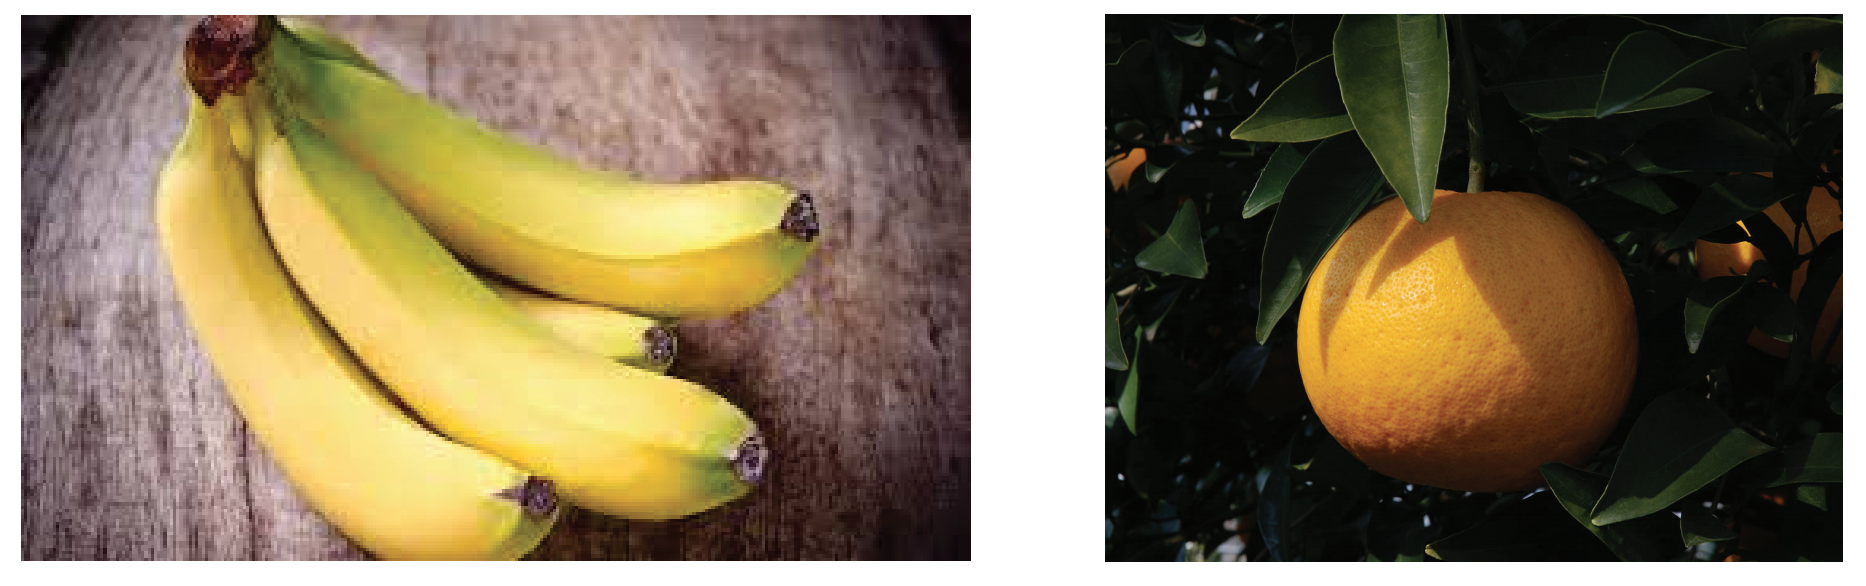
\includegraphics[scale=0.5]{fruit_examples}\caption{Example of properly centered images of four bananas against a table (left) and one orange on a tree (right).} \label{fig:robot}\end{center}\end{figure}Please keep in mind that data is an integral part of Machine Learning. A large part of research in this field relies heavily on the integrity of data in order to run algorithms. It is, therefore, vital that your data is in the proper format and is accompanied by the correct labeling not only for your grade on this section, but for the integrity of your data.
\vspace{4pt}

\noindent Note that if your compressed file is over 100 MB, you will need to downsample the images. You can use the following functions from skimage to help. 
\begin{lstlisting}
from skimage.io import imread, imsave
from skimage.transform import resize
\end{lstlisting}
\BeginSolution
%4

\EndSolution
%%%% Problem 4 Ends Here %%%%
\clearpage


%%%% Problem 5 Starts Here %%%%
\vspace{-2mm}\noindent\begin{mybox}{\begin{center}\textbf{\color{black}Problem 5: Your Own Question}\end{center}}\end{mybox}\vspace{-2mm}
\vspace{10pt}
\noindent \textbf{Write your own question, and provide a thorough solution.}
\vspace{3pt}

\noindent Writing your own problems is a very important way to really learn the material. The famous ``Bloom's Taxonomy'' that lists the levels of learning is: Remember, Understand, Apply, Analyze, Evaluate, and Create. Using what you know to create is the top-level. We rarely ask you any HW questions about the lowest level of straight-up remembering, expecting you to be able to do that yourself. (e.g. make yourself flashcards) But we don't want the same to be true about the highest level.
\vspace{3pt}

\noindent As a practical matter, having some practice at trying to create problems helps you study for exams much better than simply counting on solving existing practice problems. This is because thinking about how to create an interesting problem forces you to really look at the material from the perspective of those who are going to create the exams. 
\vspace{3pt}

\noindent Besides, this is fun. If you want to make a boring problem, go ahead. That is your prerogative. But it is more fun to really engage with the material, discover something interesting, and then come up with a problem that walks others down a journey that lets them share your discovery. You don't have to achieve this every week. But unless you try every week, it probably won't happen ever. 
\BeginSolution
%5

\EndSolution
%%%% Problem 6 Ends Here %%%%
\clearpage

%%%% Code Appendix Starts Here %%%%
\vspace{-2mm}\noindent\begin{mybox}{\begin{center}\textbf{\color{black}Code Appendix}\end{center}}\end{mybox}\vspace{-2mm}
\begin{itemize}
\item \texttt{Prob2\_total\_least\_squares: total\_least\_squares.py}
\BeginSolution
% Paste Code Between Verbatim
\begin{verbatim}

\end{verbatim}
\EndSolution
\item \texttt{Prob3\_jl\_data: jl\_lemma\_starter\_code.py}
\BeginSolution
% Paste Code Between Verbatim
\begin{verbatim}

\end{verbatim}
\EndSolution
\end{itemize}
%%%% Code Appendix Ends Here %%%%

\end{document}
%%%%% Template Ends Here %%%%%